\documentclass[12pt]{article}
\usepackage[utf8]{inputenc}
\usepackage{caption}
\usepackage{graphicx}
\usepackage{amsmath}
\usepackage{fancyhdr}
\usepackage{adjustbox}
\usepackage[most]{tcolorbox}

\usepackage{color}
\usepackage{titlesec}
\usepackage{tikz}
\usepackage{wrapfig}  
\usepackage[a4paper,top=2.8cm,bottom=0.8cm,left=2.5cm,right=2.5cm,margin=1in]{geometry}
\usepackage{xcolor}
\usepackage{enumitem}
\usepackage{setspace}
\usepackage{titling}
\usepackage{lipsum}
\usepackage{float}
\usepackage{caption}
\usepackage{subcaption}
\pagestyle{empty}
\setlength{\parindent}{0pt}
\setlength{\parskip}{0.8em}
\setstretch{1.1}
\definecolor{chapterblue}{RGB}{0,174,239} 
\definecolor{darkskyblue}{rgb}{0.0, 0.5, 1.0}
\definecolor{skyblue}{RGB}{135, 206, 235}
\usepackage{newtxtext,newtxmath}
\titleformat{\section}
  {\fontsize{67}{48}\selectfont\bfseries\color{chapterblue}}{\thesection}{1em}{}
% Title format
\titleformat{\section}
  {\normalfont\Large\bfseries\color{chapterblue}}{\thesection}{1em}{}
% Header/Footer settings
\pagestyle{fancy}
\cfoot{2019-20}
\renewcommand{\headrulewidth}{0pt}
\renewcommand{\footrulewidth}{0pt}
\begin{document}
\pagestyle{empty}
\thispagestyle{fancy}
\renewcommand{\headrulewidth}{0pt} 
\fancyhead[L]{
        
\includegraphics[width=5cm, height=2cm]{comet.jpeg} 
        }
\fancyhead[R]{
    Name: G.MADHU LATHA \\
    Batch: COMETFWC029\\
    Date: 21-may 2025
}
\begin{center}
   \vspace{5em} 
\includegraphics[width=100pt]{scanner.png} 
\end{center}

\hfill
\vspace{-4.6em}
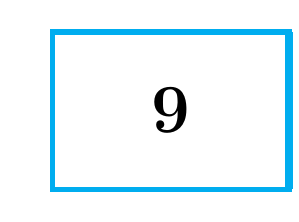
\begin{tikzpicture}
    \vspace{0em}\hspace{0.8em}\draw[line width=2pt, draw=cyan ] (0,0) rectangle (3,2); \draw[line width=3pt, draw=cyan] (3,0)--(3,2);
     \node at (1.5,1) {\textcolor{black}{\fontsize{60pt}{60pt}\selectfont \textbf{9}}};
\end{tikzpicture}
 \vspace{-0.5em}
\begin{center}
\vspace{-2em}
    {\textcolor{chapterblue}{
        \textbf{
               {\fontsize{30}{40}\selectfont S}{\fontsize{20}{34}\selectfont OME }         
           \vspace{1em} {\fontsize{30}{46}\selectfont A}{\fontsize{20}{34}\selectfont PPLICATIONS OF}\\
           {\fontsize{30}{40}\selectfont T}{\fontsize{20}{34}\selectfont RIGONOMETRY }   }
                       }
  }
\end{center}
\vspace{-2em}
\noindent

\begin{tikzpicture}
  \draw[chapterblue, line width=4pt] (0,0) -- (\linewidth,0);
\end{tikzpicture}
\section*{9.1 Introduction}
\vspace{-1em}
In the previous chapter, you have studied about trigonometric ratios. In this chapter, you will be studying about some ways in which trigonometry is used in the life around you.Trigonometry is one of the most ancient subjects studied by scholars all over the world. As we have said in Chapter 8, trigonometry was invented because its need arose in astronomy. Since then, astronomers have used it, for instance, to calculate distances from the Earth to the planets and stars. Trigonometry is also used in geography and in navigation. The knowledge of trigonometry is used to construct maps, determine the position of an island in relation to the longitudes and latitudes.
\noindent
\begin{tcolorbox}[
    colback=white,
    colframe=cyan!60!black,
    boxrule=0.6pt,
    arc=2pt,
    width=\textwidth,
    left=10pt, right=5pt, top=10pt, bottom=6pt,
    enhanced
]



\begin{minipage}[t]{0.55\textwidth}
\color{black}
\small
Surveyors have used trigonometry for centuries. One such large surveying project of the nineteenth century was the \textbf{‘Great Trigonometric Survey’}of British India for which the two largest-ever theodolites were built. During the survey in 1852, the highest mountain in the world was discovered. From a distance of over 160 km, the peak was observed from six different stations. In 1856, this peak was named after Sir George Everest, who had commissioned and first used the giant theodolites (see the figure alongside). The theodolites are now on display in the Museum of the Survey of India in Dehradun.

\end{minipage}
\hspace{7pt}
\begin{minipage}[t][5.6cm][b]{0.44\textwidth}
\centering
\textit{ \textcolor{cyan}{\textbf{A Theodolite \\}}
(Surveying instrument, which is based on the Principles of trigonometry, is used for measuring angles with a rotating telescope)}
\end{minipage}

\end{tcolorbox}
\newpage{}
\pagestyle{fancy}
\fancyhf{}
\fancyhead[L]{\textbf{Page no 196}}
\fancyhead[R]{\textbf{Mathematics}} 
\renewcommand{\headrulewidth}{0pt}
\makeatletter
\def\headrule{%
  {\color{cyan}%
   \hrule width\headwidth height 1pt \vskip-1pt}
}
\makeatother



\lhead{\textcolor{cyan}{\textbf{196}}}
\rhead{\textcolor{cyan}{\textbf{MATHEMATICS}}}
\hspace{2em}
In this chapter, we will see how trigonometry is used for finding the heights and distances of various objects, without actually measuring them.
\vspace{-2em}
\section*{9.2 Heights and Distances}
\vspace{-1em}
Let us consider Fig. 8.1 of previous chapter, which is redrawn below in Fig. 9.1
\begin{center}
\begin{figure}[h]
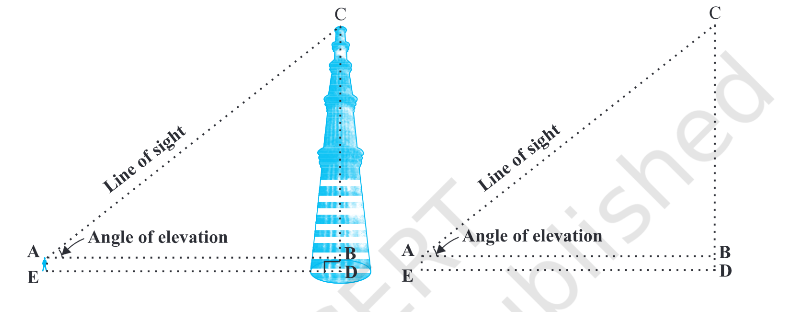
\includegraphics[width=17cm,height=8cm]{math.png}
\caption*{\textbf{\textcolor{cyan}{Fig.9.1}}}
\end{figure}
\end{center}
\vspace{-3em}
\hspace{2em}In this figure, the line AC drawn from the eye of the student to the top of the minar is called the \textit{line of sight}. The student is looking at the top of the minar. The angle BAC, so formed by the line of sight with the horizontal, is called the \textit{angle of elevation} of the top of the minar from the \textit{eye} of the student.

\hspace{2em}Thus, the \textbf{line of sight} is the line drawn from the eye of an observer to the point in the object viewed by the observer. The \textbf{angle of elevation} of the point viewed is the angle formed by the line of sight with the horizontal when the point being viewed is above the horizontal level, i.e., the case when we raise our head to look at the object (see Fig. 9.2).
\vspace{5em}\begin{center}\begin{figure}[h]
\includegraphics[width=17cm,height=10cm]{}
\caption*{\textbf{\textcolor{cyan}{Fig.9.2}}}
\end{figure}
\end{center}

\cfoot{2019-20}


\end{document}